\documentclass{article}

\usepackage[a4paper,width=150mm,top=25mm,bottom=25mm]{geometry}
\usepackage[utf8]{inputenc}
\usepackage{graphicx}
\usepackage{listings}
\usepackage{amssymb}
\usepackage{hyperref}
\usepackage{amsmath}

\title{
    {
\includegraphics{./images/logo_pk.jpg}}\\
    {Artificial Intelligence}\\
    {\large Emotion recognition with Convolutional neural networks}\\
     \small Leaded by M.Eng Kazimierz Kiełkowicz
    }
    \author{Wojciech Chmura, Konrad Krukar}
    \date{May 2020}



\begin{document}
    \maketitle
    \newpage
    \tableofcontents
    \newpage
    
    \section{Overview}
    This project will show the process of building a Convolutional Neural Network to recognize emotions on humans faces.This type of application can be useful and be applied in various systems such as security cameras.
As we know nonverbal signals sometimes say more than words.

We take two approaches: pretrained model with our final layers and our own model.

    
    \section{Introduction}
    Humans can use different forms of communications such as speech, hand gestures and emotions. Being able to understand one’s emotions and the encoded feelings is an important factor for an appropriate and correct understanding. As such systems that can recognize them, allowing for a more diverse and natural way of communication, are in great demand in many fields. It could for example help during counselling and other healthcare related fields. Other fields like surveillance or driver safety could also profit from it. Being able to detect the mood of the driver could help to detect the level of attention, so that automatic systems can adapt. There are many emotions that can be shown on human faces, but most researchers aim to identify six basic emotions, identified by Paul Ekman - anger, disgust. fear, happiness, sadness and surprise.\\

Many methods rely on extraction of the facial region. This can be realized in two ways - through manual inference or an automatic detection approach. Methods often involve the Facial Action Coding System which describes the facial expression deconstructing it into the specific action units (AU). An Action Unit is a facial action like ”raising the InnerBrow”. Multiple activation of AUs can describe the facial expression. Being able to correctly detect AUs is a helpful step, since it allows making a statement about the activation level of the corresponding emotion, but detecting handcrafted facial landmarks can be hard, as the distance between them differs depending on the person. Also, it is significantly harder to determine the facial features of a person when only part of their face is visible or if the lighting conditions are poor.\\

Our approach uses Convolutional Neural Networks, which is a special kind of ANN and have been shown to work well as feature extractor when using images as input and are real-time capable. This allows for the usage of the raw input images without any pre- or post- processing.\\
    
    
    \newpage
    \section{Convolutional Neural Networks}
    A convolutional neural network (CNN) is a class of deep neural networks, most commonly applied to analyzing visual imagery. Convolutional networks were inspired by biological processes - pattern between neurons resembles the organization of the animal visual cortex. A convolutional neural network consists of an input and an output layer, as well as multiple hidden layers. The hidden layers of a CNN typically consist of a series of convolutional layers, subsequently followed by additional convolutions such as pooling layers, fully connected layers and normalization layers.\\

\subsection{Convolutional Layer}
The convolutional layer is the core building block of a CNN. The layer's parameters consist of a set of learnable kernels, which have a small receptive field, defined by a width and height. Kernel extends through the full depth of the input volume. During the forward pass, each filter is computing the dot product between the entries of the filter and the input and producing a 2-dimensional activation map of that filter. Stacking the activation maps for all filters along the depth dimension forms the full output volume of the convolution layer. Such a two-dimensional output array from this operation is called a “feature map“. Once a feature map is created, we can pass each value in the feature map through a nonlinearity, such as a ReLU, much like we do for the outputs of a fully connected layer.
\\Let fk be the filter with a kernel size n x m applied to the input x. n x m is the number of input connections each CNN neuron has. The resulting output of the layer calculates as follows:
\begin{large}
    $$C(x_{u,v}) = \sum_{i = \frac{n}{2}}^{\frac{n}{2}} \sum_{i = \frac{m}{2}}^{\frac{m}{2}} f_{k}(i, j)x_{u-i,v-j} $$
\end{large}
In summary, we have a input, such as an image of pixel values, and we have a kernel, which is a set of weights, and the kernel is systematically applied to the input data to create a feature map.

\subsection{ReLU}
ReLU is the abbreviation of rectified linear unit, which applies the non-saturating activation function\\
\begin{center}
    \begin{large}
        $f(x)=\max(0,x)$
    \end{large} \\
\end{center}
It effectively removes negative values from an activation map by setting them to zero. It increases the nonlinear properties of the decision function and of the overall network without affecting the receptive fields of the convolution layer.\\
Other functions could be also used to increase nonlinearity, but ReLU is often preferred to other functions because it trains the neural network several times faster without a significant penalty to generalization accuracy

\subsection{Pooling layer}
Another important concept of CNNs is pooling, which is a form of non-linear down-sampling. There are several non-linear functions to implement pooling among which max pooling is the most common. It partitions the input image into a set of non-overlapping rectangles and, for each such sub-region, outputs the maximum. The most common form is a pooling layer with filters of size 2x2 applied with a stride of 2 downsamples every depth slice in the input by 2 along both width and height, discarding 75 %
of the activations. Every MAX operation would in this case be taking a max over 4 numbers (little 2x2 region in some depth slice). \\
In addition to max pooling, the pooling units can also perform other functions, such as average pooling or even L2-norm pooling. Average pooling was often used historically but has recently fallen out of favor compared to the max pooling operation, which has been shown to work better in practice.\\

\subsection{Max Pooling}
Max Pooling: Max Pooling reduces the input by applying the maximum function over the input xi. Let m be the size of the filter, then the output calculates as follows:
This layer features translational invariance with respect to the filter size.
\begin{center}
    \begin{large}
        $$M(x_i)=max\left \{X_{i+k,i+l}||k|\leq \frac{m}{2},|l|\leq \frac{m}{2}k,l\in \mathbb{N}\right \}$$
    \end{large} \\
\end{center}

\subsection{Fully connected layer}
The output from the convolution layer was a 2D matrix. Ideally, we would want each row to represent a single input image. In fact, the fully connected layer can only work with 1D data. Hence, the values generated from the previous operation are first converted into a 1D format.\\
\begin{center}
    \begin{large}$$
        \begin{Bmatrix}
         9, 32 \\
         14,26
        \end{Bmatrix}
        \rightarrow
        \begin{Bmatrix}
         9 \\ 32 \\ 14 \\26
        \end{Bmatrix}$$
    \end{large} \\
\end{center}
Once the data is converted into a 1D array, it is sent to the fully connected layer. All of these individual values are treated as separate features that represent the image. The fully connected layer performs two operations on the incoming data – a linear transformation and a non-linear transformation.\\    
    
    \newpage
    \section{Dataset description}
    Data that we got is in one *.csv file with two columns:
\begin{itemize}
  \item number of emotion \\
    in rage 0 - 6:
    \begin{itemize}
        \item 0 - angry
        \item 1 - disgust
        \item 2 - fear
        \item 3 - happy
        \item 4 - sad
        \item 5 - surprise
        \item 6 - neutral
    \end{itemize}
  \item string of pixels \\
    Pixels are in one long string (2304 of them), they are in gray scale 0 - 255.\\
    We need to preprocess them into array of 48x48x1 that will could be reorganised as an picture also we will change to rage to 0 - 1 scale - by dividing via 255
    \lstinputlisting[language=Python]{../Model/DataProcess.py}

\end{itemize}

    
    \newpage
    \section{Approach 1: Transfer learning with VGG16}
    At the beginning we decided to use transfer learning: pretrained VGG16 model with our additional final layers.
 
    	\subsection{VGG16 Description}
    	\includegraphics[scale=0.5]{images/modelOne/vgg16.png}
VGG16 is a convolutional neural network model proposed by K. Simonyan and A. Zisserman from the University of Oxford for ILSVRC-2014 competition. This model achieves 92.7% top-5 test accuracy on ImageNet dataset which contains 14 million images belonging to 1000 classes.//
\\It is considered to be one of the excellent vision model architecture till date. Most unique thing about VGG16 is that instead of having a large number of hyper-parameter they focused on having convolution layers of very small receptive fields - 3x3 filter with a stride 1. It also always uses same padding and maxpool layers of 2x2 filters of stride 2. It follows this arrangement of convolution and max pool layers consistently throughout the whole architecture. In the end it has 2 fully connected layers followed by a softmax for output. The 16 in VGG16 refers to it has 16 layers that have weights. This network is a pretty large network and it has about 138 million parameters. ~\cite{vgg16desc}

    	
    	\newpage
    	\subsection{Model building}
    	We decided to use pre-traind VGG16 model, without its top two layers.\\

{\includegraphics[scale=0.5]{./images/vgg16.png}} \\

VGG16 is a convolutional neural network model proposed by K. Simonyan and A. Zisserman
from the University of Oxford in the paper “Very Deep Convolutional Networks
for Large-Scale Image Recognition”. The model achieves 92.7%
top-5 test accuracy in ImageNet, which is a dataset of over 14 million
images belonging to 1000 classes. It was one of the famous model submitted
to ILSVRC-2014. It makes the improvement over AlexNet by replacing large
kernel-sized filters (11 and 5 in the first and second convolutional layer,
respectively) with multiple 3×3 kernel-sized filters one after another. VGG16
was trained for weeks and was using NVIDIA Titan Black GPU’s.

In Keras it's really easy to implemnt this model and freeze layers to non-trainable (In code in "Implementaion" section)
Our VGG model looks lika this:\\

{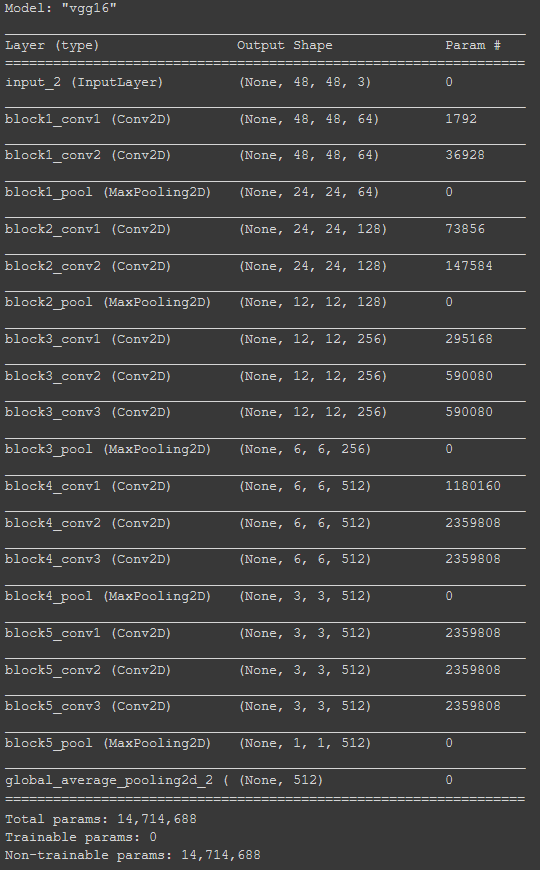
\includegraphics[scale=0.75]{./images/vggNT.png}} \\


    
    	\newpage
    	\subsection{Data Preprocessing}
    	Images must be preprocessed into a 48x48 arrays, so that it could be reorganised as a picture, also change the range from 0 -255 to 0 - 1
and add third dimension.
\lstinputlisting[language=Python, firstline=25, lastline=42]{../Model/two/OwnCNN.py}
Split dataset into the training part and testing part:
\lstinputlisting[language=Python, firstline=16, lastline=19]{../Model/two/OwnCNN.py}
~\cite{repo}
    	
    	\newpage
    	\subsection{Code implementation}
    	\lstinputlisting[language=Python, firstline=58, lastline=92]{../Model/two/OwnCNN.py}
~\cite{repo}
    
    	\newpage
    	\subsection{Results}
    	We have trained our model with a batch size of 128 with.
Accuracy:
\begin{itemize}
      \item Training Set:
        \begin{itemize}
            \item First epochs: 24,8\%
            \item Last epoch: 93,6\%
        \end{itemize}
      \item Test Set:
        \begin{itemize}
            \item First epochs: 24,9\%
            \item Last epoch: 61,3\%
        \end{itemize}
\end{itemize}
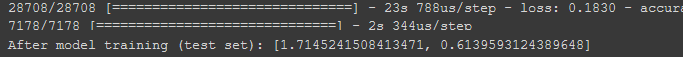
\includegraphics[scale=0.9]{images/modelTwo/evalutaionTwo.png}
Test/Validation Set result is much batter then in prevoius model.\\
\\
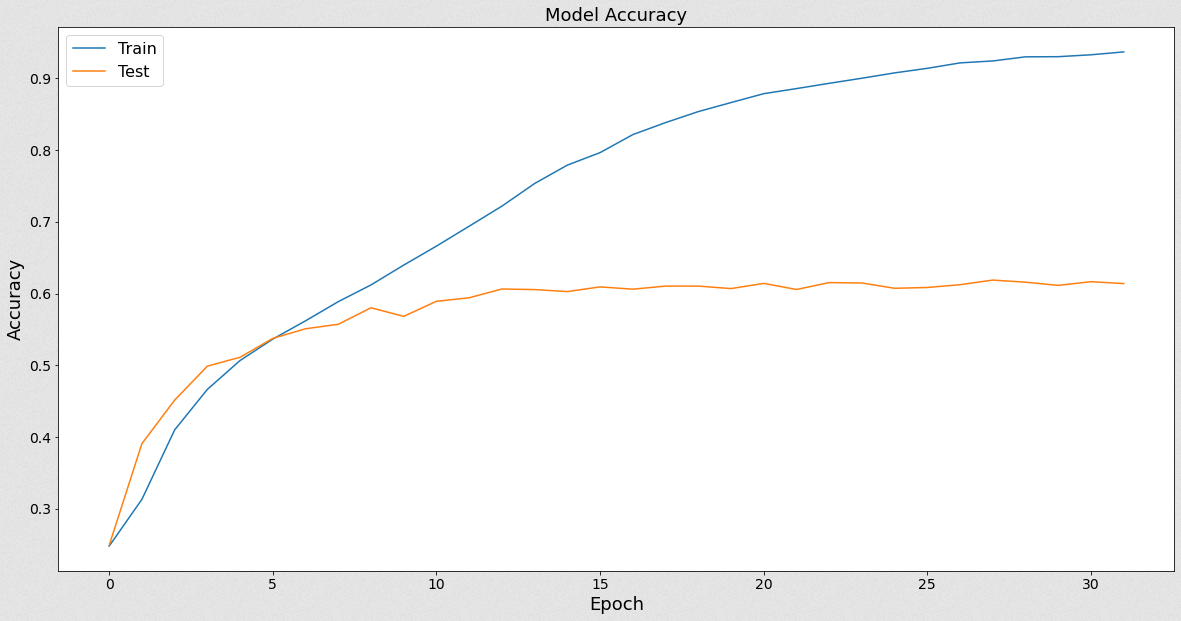
\includegraphics[scale=0.5]{images/modelTwo/accTwo.png}
Accuracy rises as expected.\\
\newpage
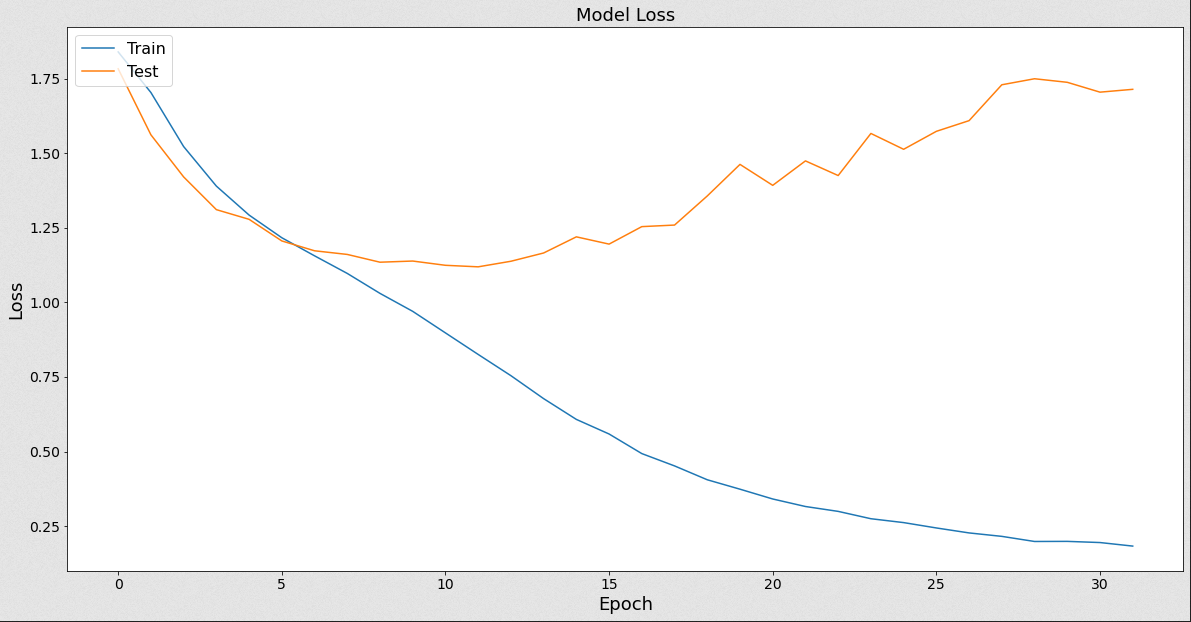
\includegraphics[scale=0.5]{images/modelTwo/lossTwo.png}
As we can see model is over-fitting again but much less.\\
\\
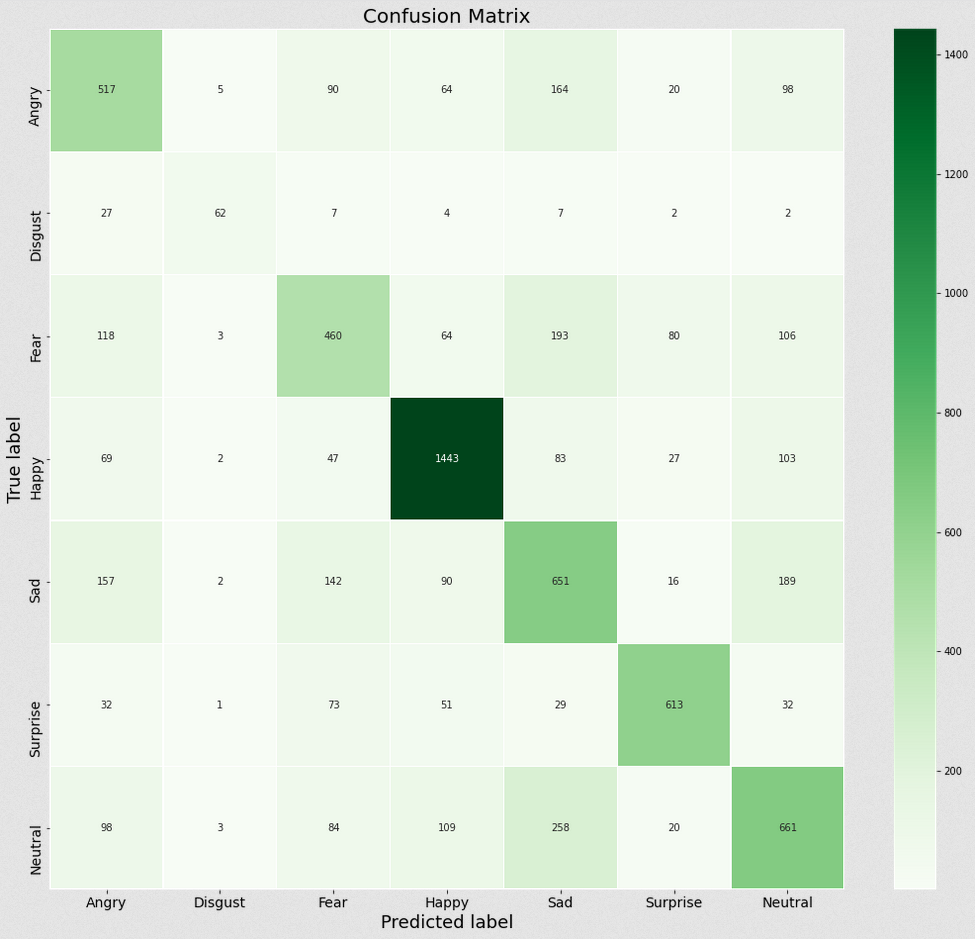
\includegraphics[scale=0.60]{images/modelTwo/matrixTwo.png}
Confusion matrix shows us mistakes that model made.\\
\\
Here we have some examples:
\begin{itemize}
    \item Correctly predicted images\\
            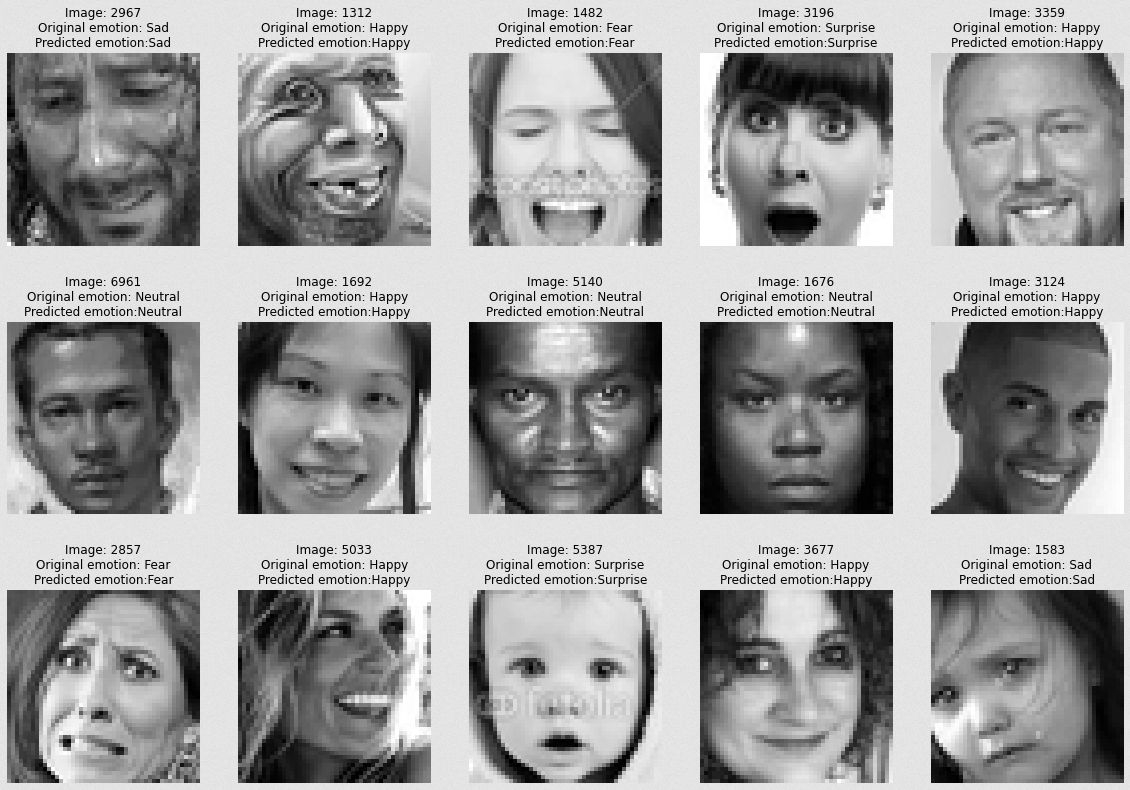
\includegraphics[scale=0.50]{images/modelTwo/trueTwo.png}
    \item Wronly predicted images\\
            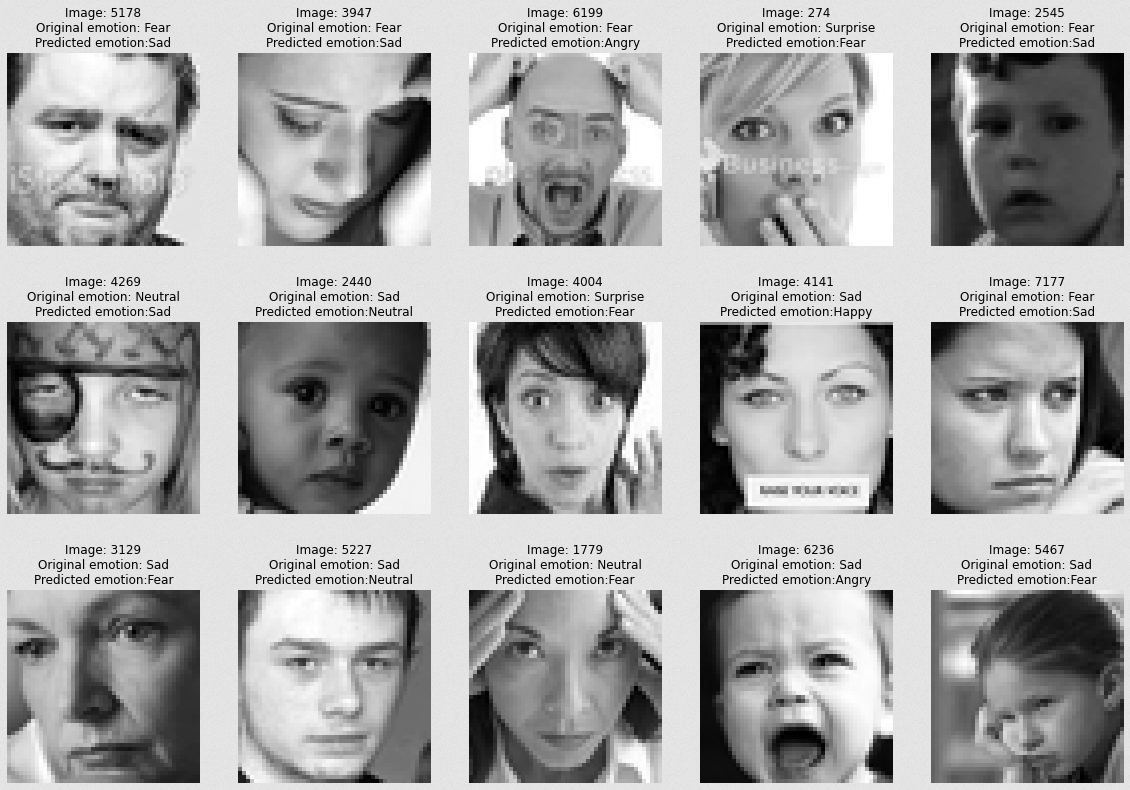
\includegraphics[scale=0.50]{images/modelTwo/falseTwo.png}
\end{itemize}

    	
    \newpage
    \section{Approach 2: Our own CNN model}
    Seeing the results of the previous model, we decided to create our own CNN.

    	    	
    	\subsection{Model building}
    	We decided to use pre-traind VGG16 model, without its top two layers.\\

{\includegraphics[scale=0.5]{./images/vgg16.png}} \\

VGG16 is a convolutional neural network model proposed by K. Simonyan and A. Zisserman
from the University of Oxford in the paper “Very Deep Convolutional Networks
for Large-Scale Image Recognition”. The model achieves 92.7%
top-5 test accuracy in ImageNet, which is a dataset of over 14 million
images belonging to 1000 classes. It was one of the famous model submitted
to ILSVRC-2014. It makes the improvement over AlexNet by replacing large
kernel-sized filters (11 and 5 in the first and second convolutional layer,
respectively) with multiple 3×3 kernel-sized filters one after another. VGG16
was trained for weeks and was using NVIDIA Titan Black GPU’s.

In Keras it's really easy to implemnt this model and freeze layers to non-trainable (In code in "Implementaion" section)
Our VGG model looks lika this:\\

{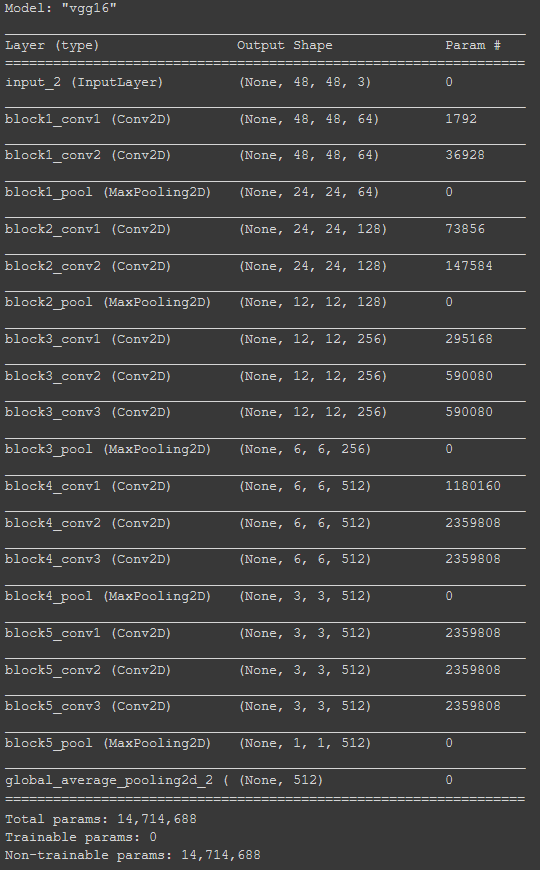
\includegraphics[scale=0.75]{./images/vggNT.png}} \\


    
    	\newpage
    	\subsection{Data Preprocessing}
    	Images must be preprocessed into a 48x48 arrays, so that it could be reorganised as a picture, also change the range from 0 -255 to 0 - 1
and add third dimension.
\lstinputlisting[language=Python, firstline=25, lastline=42]{../Model/two/OwnCNN.py}
Split dataset into the training part and testing part:
\lstinputlisting[language=Python, firstline=16, lastline=19]{../Model/two/OwnCNN.py}
~\cite{repo}
    	
    	\newpage
    	\subsection{Code implementation}
    	\lstinputlisting[language=Python, firstline=58, lastline=92]{../Model/two/OwnCNN.py}
~\cite{repo}
    
    	\newpage
    	\subsection{Results}
    	We have trained our model with a batch size of 128 with.
Accuracy:
\begin{itemize}
      \item Training Set:
        \begin{itemize}
            \item First epochs: 24,8\%
            \item Last epoch: 93,6\%
        \end{itemize}
      \item Test Set:
        \begin{itemize}
            \item First epochs: 24,9\%
            \item Last epoch: 61,3\%
        \end{itemize}
\end{itemize}
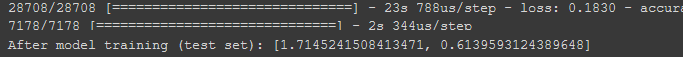
\includegraphics[scale=0.9]{images/modelTwo/evalutaionTwo.png}
Test/Validation Set result is much batter then in prevoius model.\\
\\
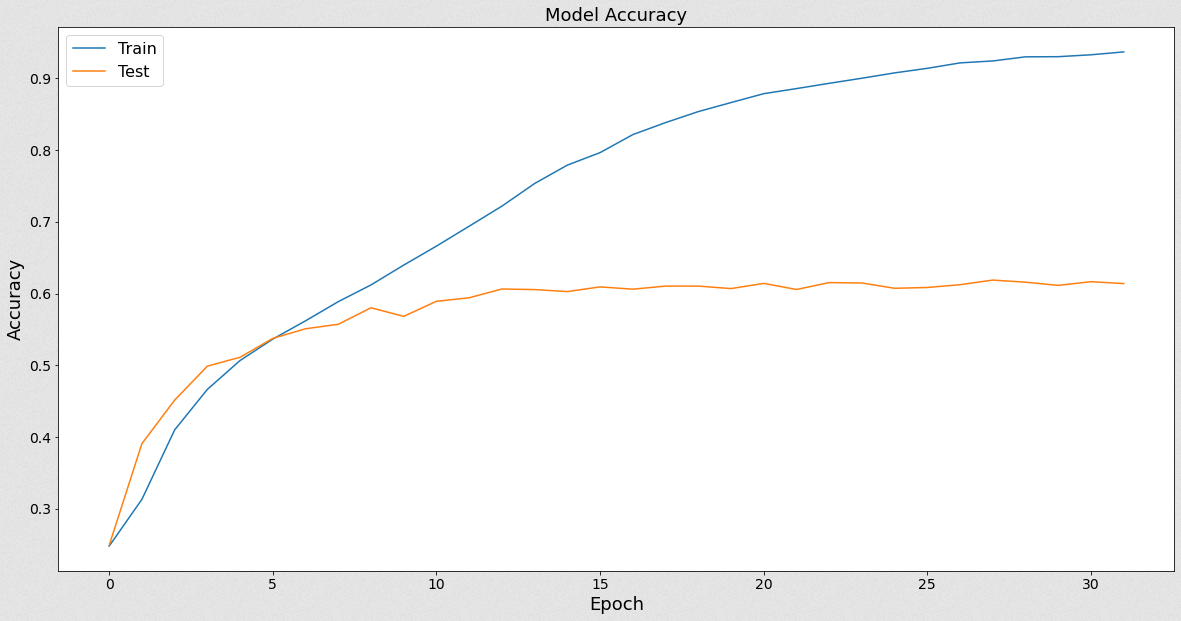
\includegraphics[scale=0.5]{images/modelTwo/accTwo.png}
Accuracy rises as expected.\\
\newpage
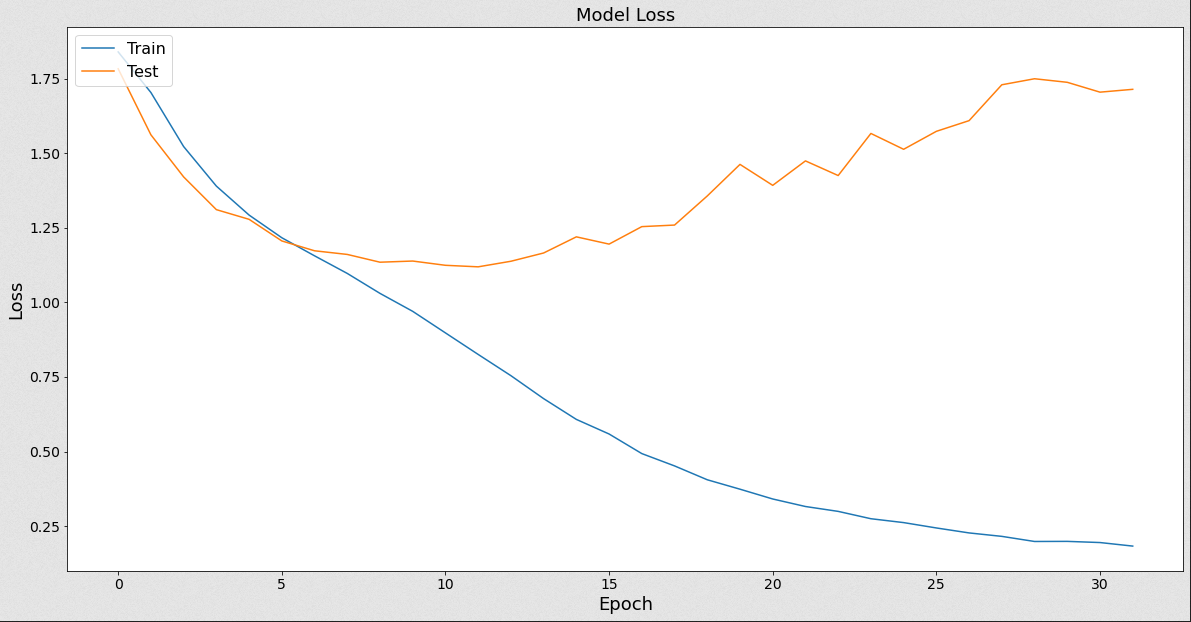
\includegraphics[scale=0.5]{images/modelTwo/lossTwo.png}
As we can see model is over-fitting again but much less.\\
\\
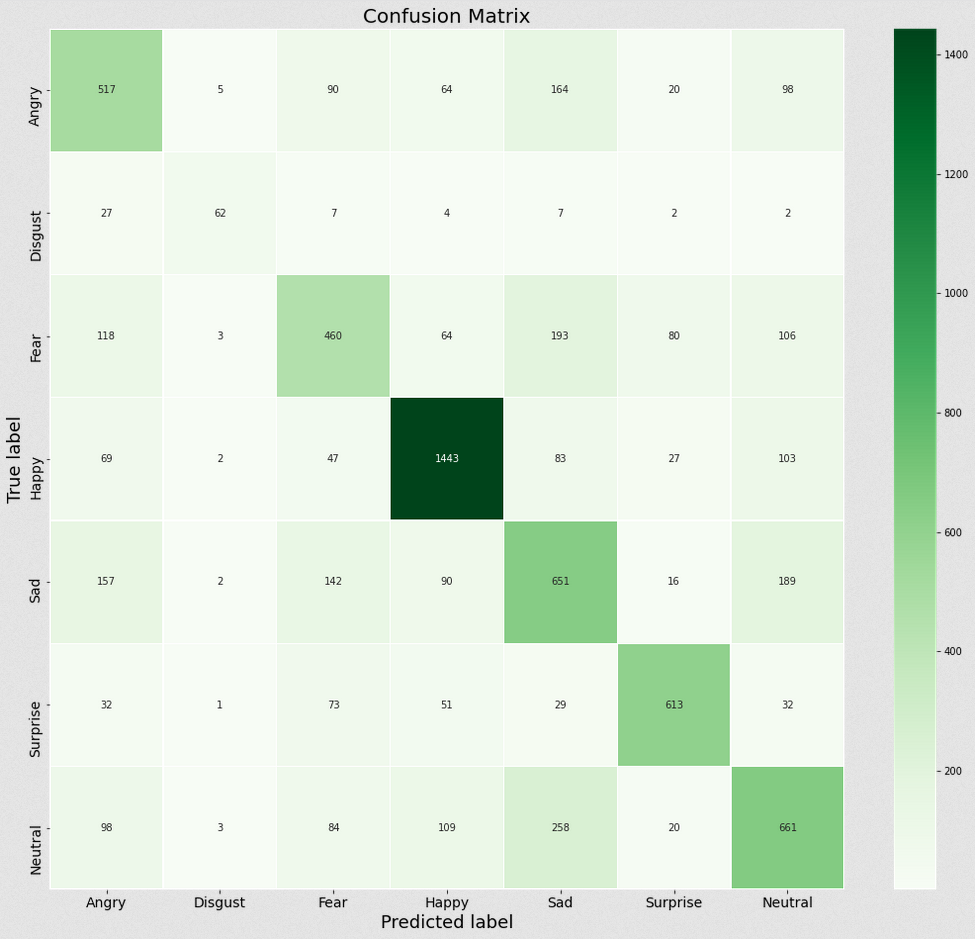
\includegraphics[scale=0.60]{images/modelTwo/matrixTwo.png}
Confusion matrix shows us mistakes that model made.\\
\\
Here we have some examples:
\begin{itemize}
    \item Correctly predicted images\\
            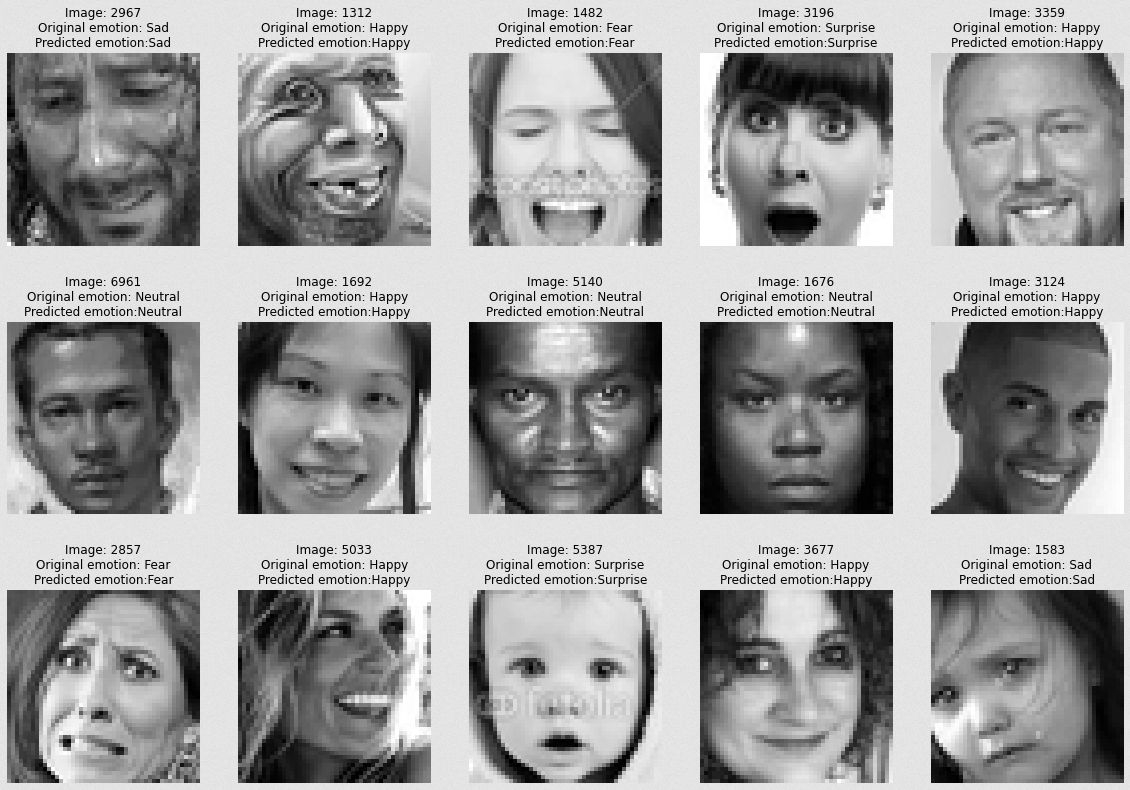
\includegraphics[scale=0.50]{images/modelTwo/trueTwo.png}
    \item Wronly predicted images\\
            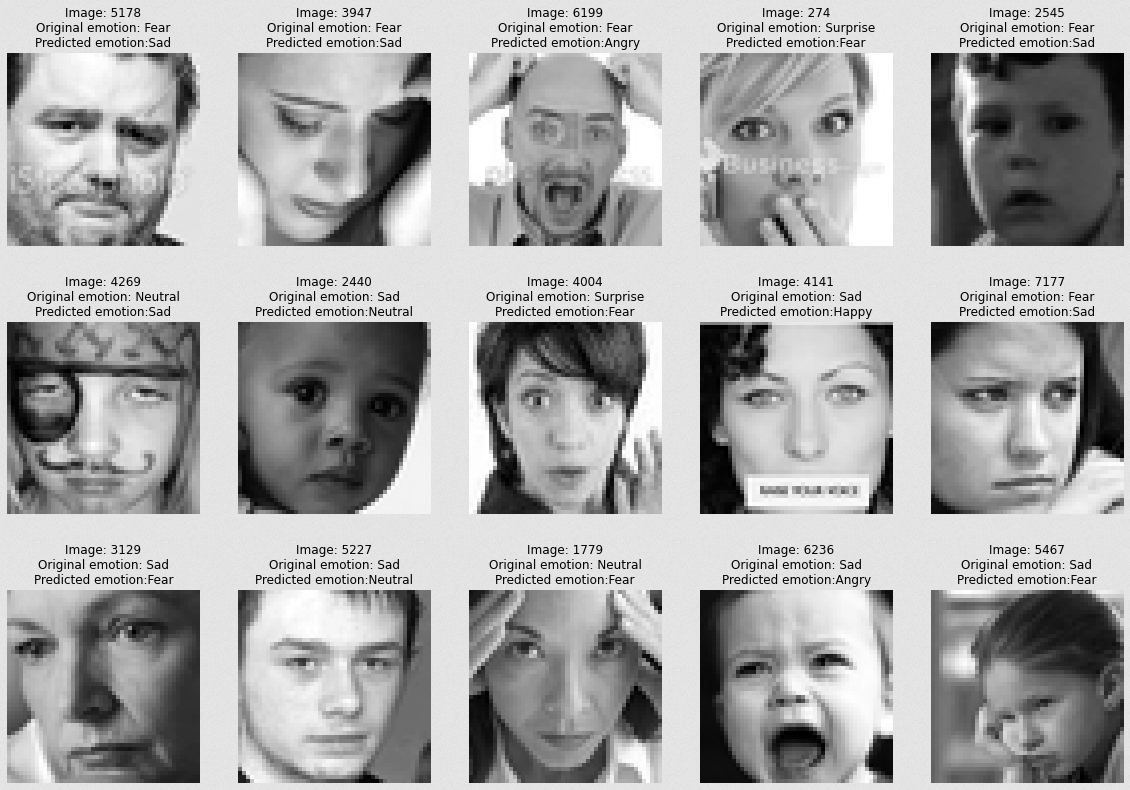
\includegraphics[scale=0.50]{images/modelTwo/falseTwo.png}
\end{itemize}


    \bibliographystyle{plain}
    \bibliography{ref}
\end{document}
